\subsection{De Turingmachine als herkenner en beslisser}

\vspace{0.5cm}

\begin{theo}[Turingmachine]{Turingmachine}
    Een \textbf{Turingmachine} is een 7-tal $(Q, \Sigma, \Gamma, \delta, q_0, q_{a}, q_{r})$ waarbij $Q, \Sigma, \Gamma$ eindige verzamelingen zijn en 
    
    \vspace{0.3cm}\begin{minipage}{0.56\textwidth}
        \begin{itemize}
            \item $Q$ is een verzameling toestanden
            \item $\Sigma$ is het input alfabet dat $\#$ niet bevat
            \item $\Gamma$ is het tape alfabet waarbij $\Sigma \subset \Gamma$ en $\# \in \Gamma$
            \item $q_s$ is de starttoestand
            \item $q_a$ is de accepterende eindtoestand
            \item $q_r$ is de verwerpende eindtoestand, verschillend van $q_a$
            \item $\delta$ is de transitiefunctie: een totale functie met signatuur
            \begin{equation*}
                Q \times \Gamma \rightarrow Q \times \Gamma \times \{L, R, S\}
            \end{equation*}
        \end{itemize}
    \end{minipage}
    \hspace{0.2cm}\begin{minipage}{0.4\textwidth}
        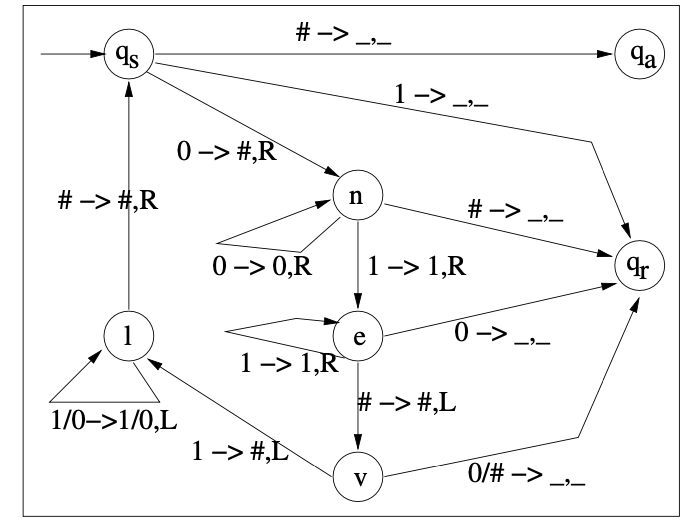
\includegraphics[scale = 0.27]{Images/TuringmachineEx.png}
    \end{minipage}
\end{theo}

% \begin{theo}[Herkennen]{Herkennen}
%     Een Turingmachine TM \textbf{herkent} een taal $L$
% \end{theo}

\begin{theo}[Turing-herkenbare taal]{Turing-herkenbare taal}
    Een taal L is \textbf{Turing-herkenbaar} als er een Turingmachine TM bestaat zodanig dat
    \begin{equation*}
        L = L_{\text{TM}}.
    \end{equation*}
    \textbf{Opmerking:} $\infty_{\text{TM}}$ is niet leeg: voor elke string niet in $L$ gaat de machine in een lus.
\end{theo}

\begin{theo}[Turing-beslisbare taal]{Turing-beslisbare taal}
    Een taal L is \textbf{Turing-beslisbaar} als er een Turingmachine TM bestaat zodanig dat
    \begin{equation*}
        L = L_{\text{TM}} \text{ en } \infty_{\text{TM}} = \emptyset.
    \end{equation*}
    \vspace{-0.3cm}
\end{theo}

\begin{theo}[Co-herkenbaar/co-beslisbaar]{Co-herkenbaar/co-beslisbaar}
    Een taal $L$ is co-herkenbaar/co-beslisbaar als $\overline{L}$ herkenbaar/beslisbaar is.
\end{theo}

\newpage

\begin{lem}[Turing-beslisbaarheid en Turing-herkenbaarheid]{Turing-beslisbaarheid en Turing-herkenbaarheid}
    \begin{enumerate}
        \item Als een taal $L$ beslisbaar is, dan is $L$ co-beslisbaar.
        \item Als een taal $L$ herkenbaar en co-herkenbaar is, dan is $L$ beslisbaar.
        \item Er bestaat een taal die niet herkenbaar is.
    \end{enumerate}
\end{lem}

\begin{prf}[Turing-beslisbaarheid en Turing-herkenbaarheid]{Turing-beslisbaarheid en Turing-herkenbaarheid}
    \begin{enumerate}
        \item 
            Verwissel de rol van $q_a$ en $q_r$ in de Turingmachine die $L$ beslist.
        \item 
            Laat $M_1$ de machine zijn die $L$ herkent, en $M_2$ de machine die $\overline{L}$ herkent. De idee is nu dat we $M_1$ en $M_2$ samen laten lopen als een nieuwe machine $M$, in parallel: zodra $M_1$ accepteert, dan accepteert $M$, en zodra $M_2$ accepteert, dan verwerpt $M$. $M_1$ en $M_2$ kunnen niet samen accepteren, en voor elke string zal minstens één van de machines $M_1$ en $M_2$ stoppen p in zijn aanvaardende toestand. $M$ beslist $L$.
        \item 
            Het bewijs steunt op het begrip kardinaliteit: we weten van vroeger dat het aantal Turingmachines aftelbaar oneindig is. We weten ook dat elke Turingmachine juist één taal herkent. En tenslotte weten we ook dat het aantal talen niet-aftelbaar oneindig is, want de verzameling talen is $\mathcal{P}(\Sigma^*)$. Bijgevolg bestaat een niet-herkenbare taal. In feite is daarmee zelfs bewezen dat er niet-aftelbaar veel niet-herkenbare talen bestaan. Meer nog: bijna alle talen zijn niet-herkenbaar!
    \end{enumerate}
\end{prf}